\section{Result}
\subsection{Part 1}
In 

Wavelength white LED: 454.17 nm 
integration time 70 ms 
averaging every 10th measurements

\begin{figure}[H]
    \centering
    \subfloat[Spring]{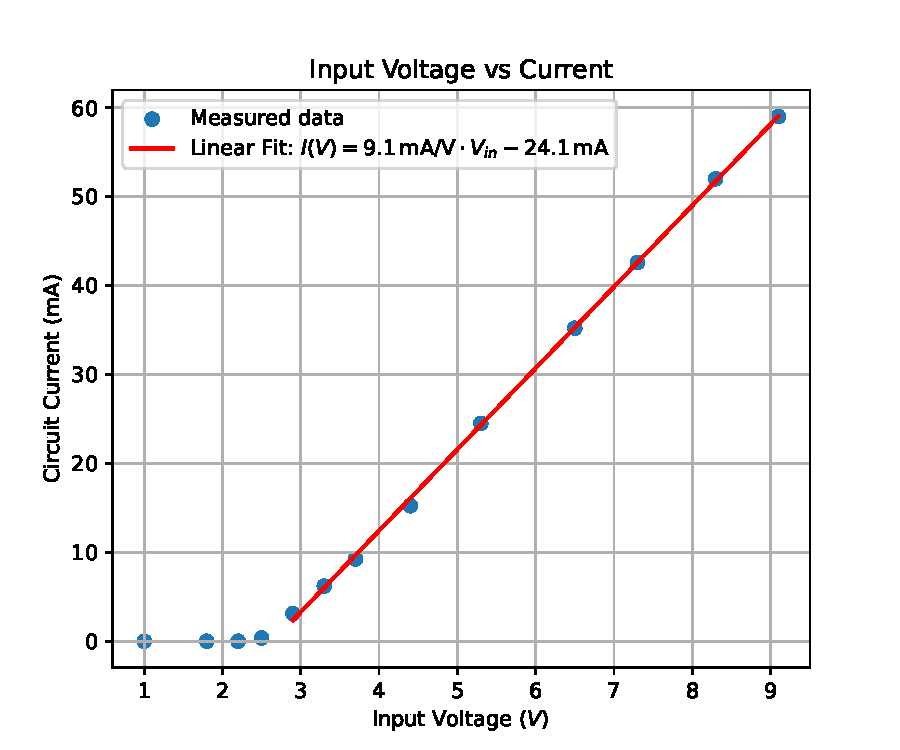
\includegraphics[width=0.49\textwidth]{Figures/part1(a).pdf} \label{fig:a}}
    \hfill
    \subfloat[Summer]{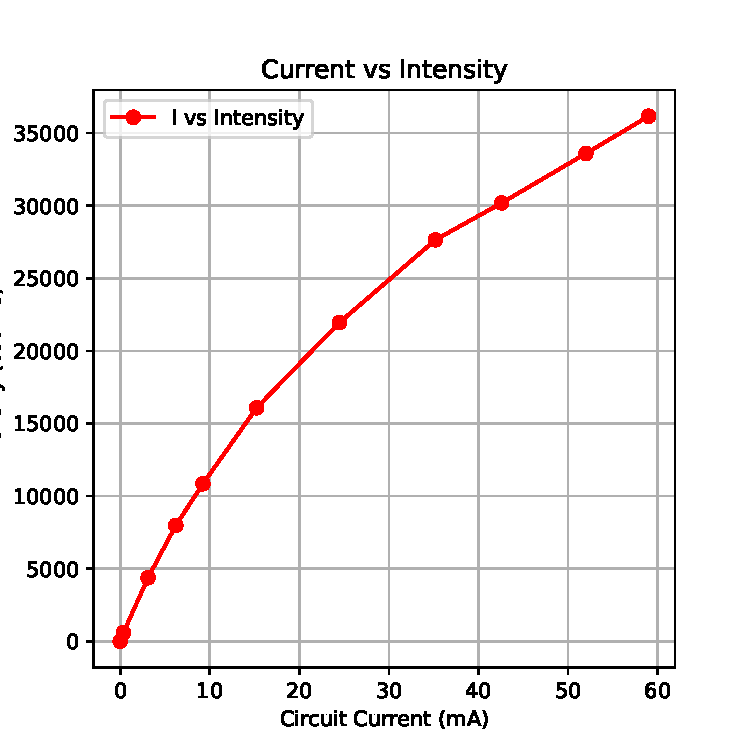
\includegraphics[width=0.49\textwidth]{Figures/part1(b).pdf} \label{fig:b}}
    
    \vspace{0.5cm}
    
    \subfloat[Autumn]{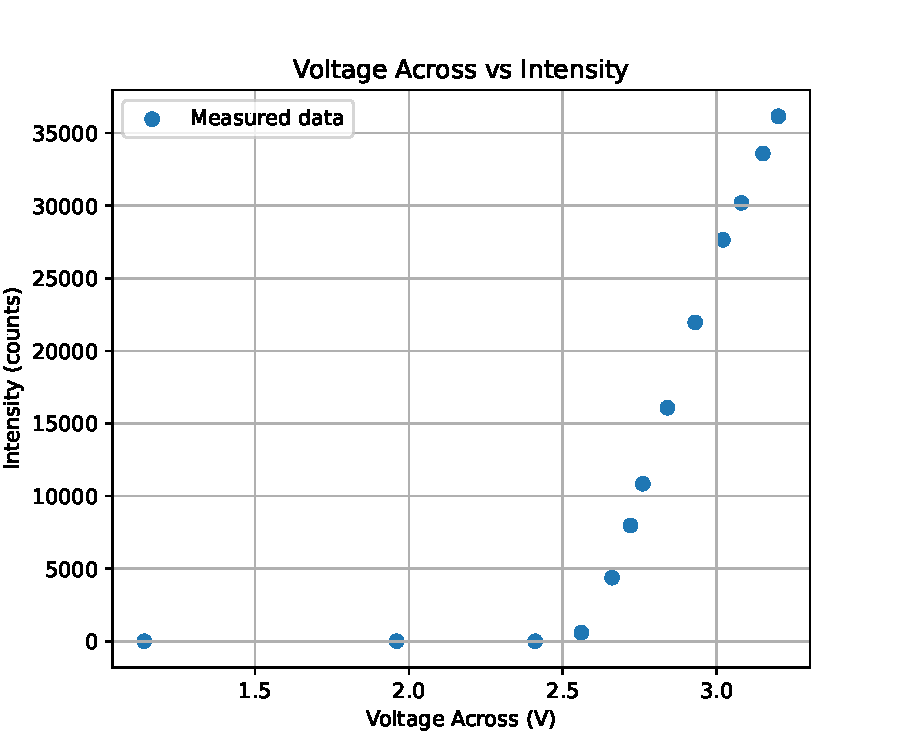
\includegraphics[width=0.49\textwidth]{Figures/part1(c).pdf} \label{fig:c}}

    
    \caption{Histograms for different seasons.}
    \label{fig:part1}
\end{figure}


\subsection{Part 2}

\begin{figure}[H]
    \centering
    \subfloat[Spring]{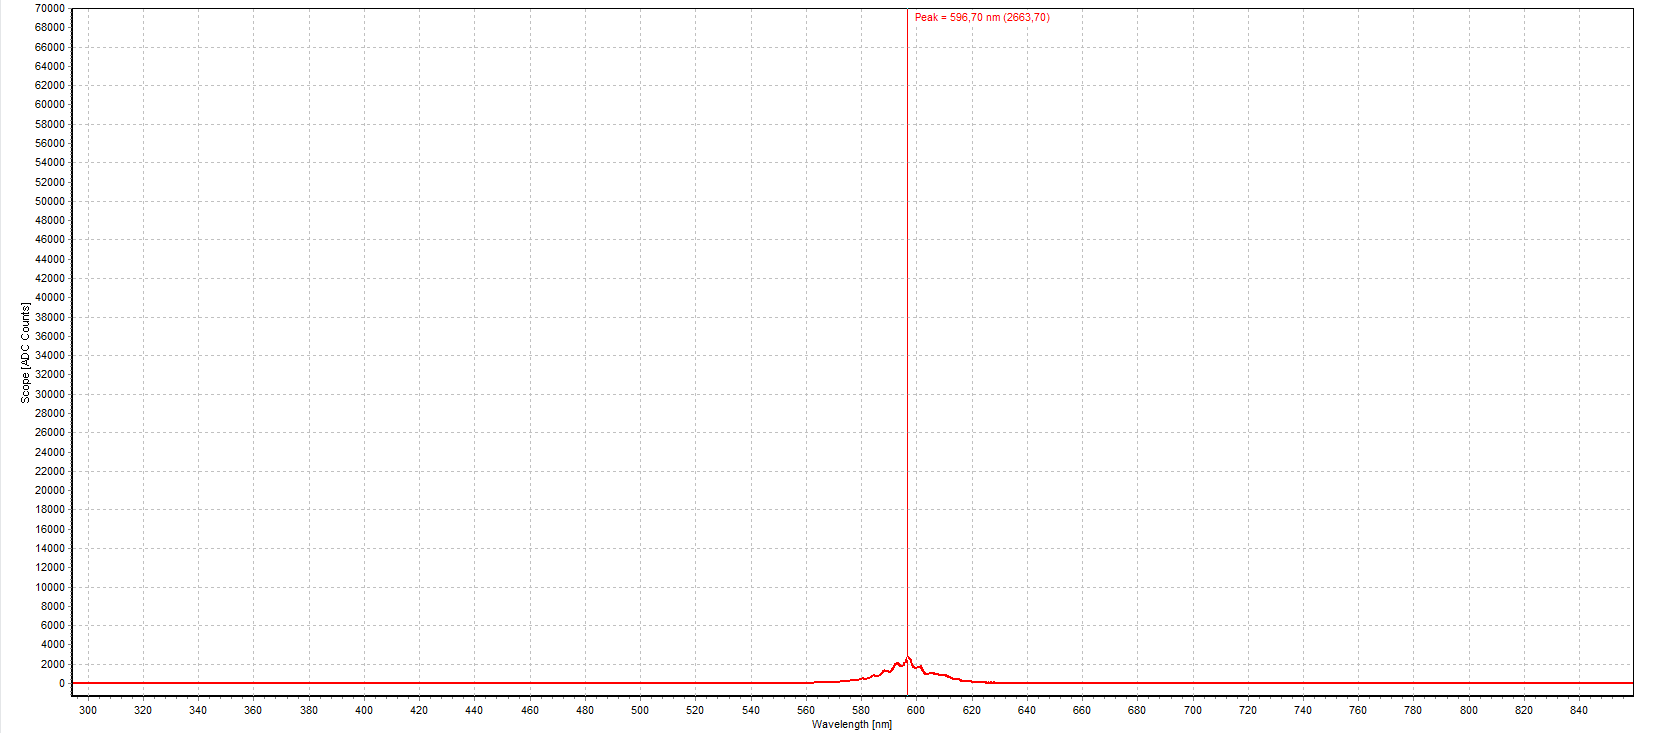
\includegraphics[width=0.9\textwidth]{Figures/Part2_before.png} \label{fig:before}}
    \hfill
    \subfloat[Summer]{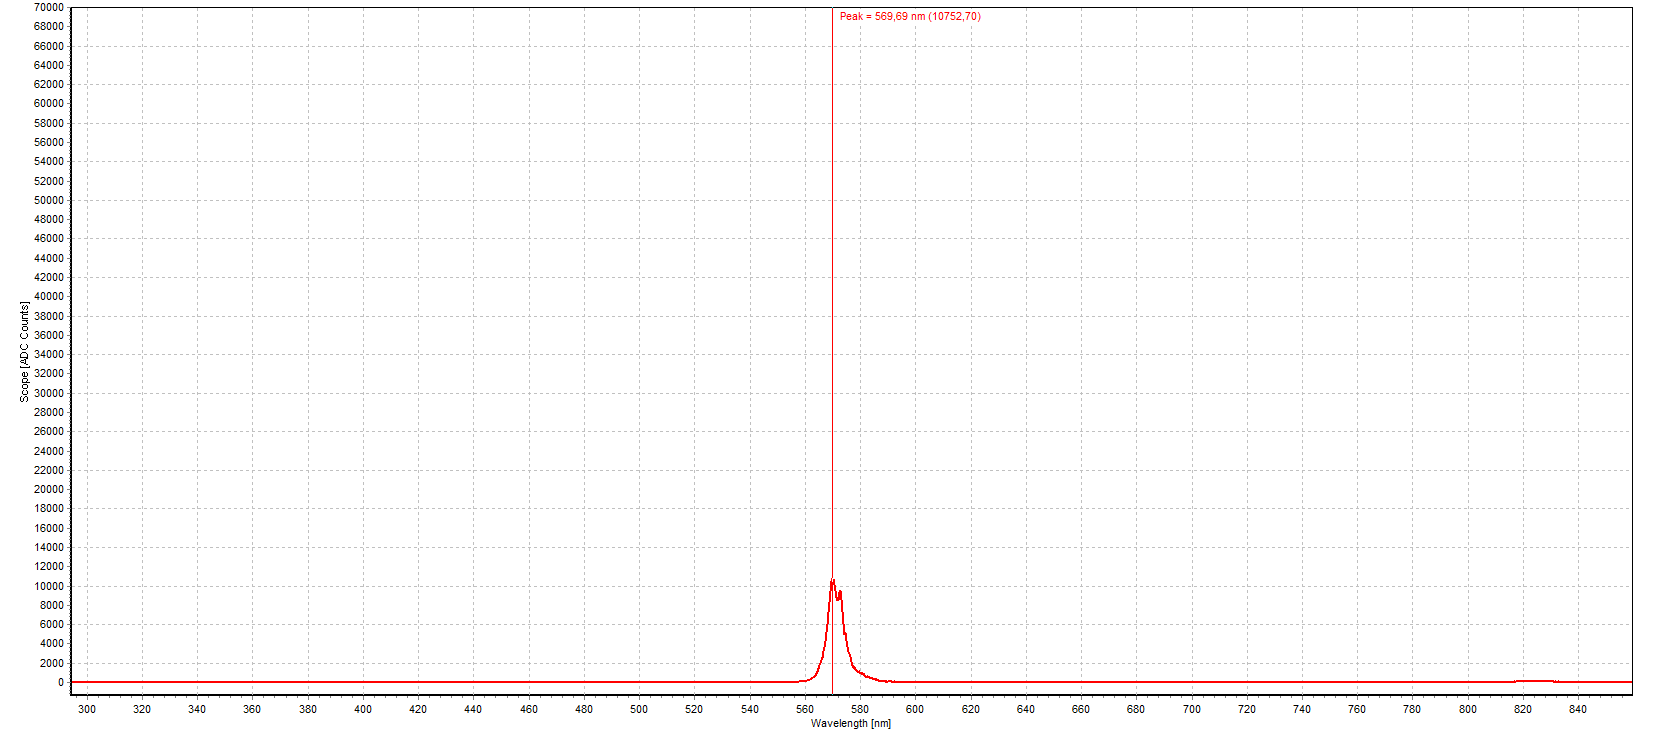
\includegraphics[width=0.9\textwidth]{Figures/Part2_after.png} \label{fig:after}}
    \caption{...}
    \label{fig:part2}
\end{figure}

Wavelength white LED: 596.85 nm 
integration time 2 ms 
averaging every 10th measurements

Before: V\textsubscript{in} was 5.0 V, V\textsubscript{across} 2.06 V, I\textsubscript{circuit} 30.8 mA and the intensity 2663.70

After: V\textsubscript{in} was 5.0 V, V\textsubscript{across} 4.44 V, I\textsubscript{circuit} 7.7 mA and the intensity 10752.70


\subsection{Part 3}

\begin{table}[H]
    \centering
    \begin{tabular}{@{}llll@{}}
    \toprule
    Detector/Emitter & Red    & Green     & Blue      \\ \midrule
    Red              & Output & No output & No output \\
    Green            & Output & Output    & No output \\
    Blue             & Output & Output    & Output    \\ \bottomrule
    \end{tabular}
    \caption{tab:part3}
\end{table}